\documentclass[tikz,border=2pt]{standalone}
\usepackage{amsmath}
\usepackage{pgfplots}
\pgfplotsset{compat=1.18}
\usetikzlibrary{arrows.meta}
\begin{document}
% Subsetting by position: x[c(1, 3)] keeps positions 1 and 3, x[-c(1, 3)] drops them;
% in A = matrix(1:12, nrow = 4), A[1, 3] = 9 and A[, 1] = (1, 2, 3, 4).
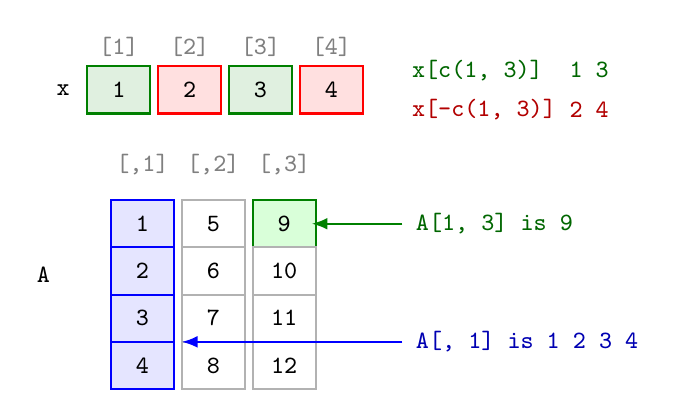
\begin{tikzpicture}[font=\small, >={Latex[length=2mm]},
  cell/.style={draw, thick, minimum width=8mm, minimum height=6mm, inner sep=0pt, font=\small\ttfamily, text=black}]
  % vector part
  \node[anchor=east] at (0.4,3.6) {\texttt{x}};
  \foreach \v/\col [count=\i] in {1/green!50!black,2/red,3/green!50!black,4/red} {
    \node[cell, draw=\col, fill=\col!12] at (0.9*\i,3.6) {\v};
    \node[gray, font=\small\ttfamily] at (0.9*\i,4.15) {[\i]};
  }
  \node[anchor=west, font=\small\ttfamily, green!40!black] at (4.5,3.85) {x[c(1, 3)]};
  \node[anchor=west, font=\small\ttfamily, green!40!black] at (6.5,3.85) {1 3};
  \node[anchor=west, font=\small\ttfamily, red!70!black] at (4.5,3.35) {x[-c(1, 3)]};
  \node[anchor=west, font=\small\ttfamily, red!70!black] at (6.5,3.35) {2 4};
  % matrix part
  \node[anchor=east] at (0.15,1.25) {\texttt{A}};
  \foreach \c in {1,2,3} {
    \node[gray, font=\small\ttfamily] at (0.3+0.9*\c,2.65) {[,\c]};
    \foreach \r in {1,2,3,4} {
      \pgfmathtruncatemacro{\v}{\r+4*(\c-1)}
      \ifnum\c=1
        \node[cell, draw=blue, fill=blue!10] at (0.3+0.9*\c,2.5-0.6*\r) {\v};
      \else
        \ifnum\r=1 \ifnum\c=3
          \node[cell, draw=green!50!black, fill=green!15] at (0.3+0.9*\c,2.5-0.6*\r) {\v};
        \else
          \node[cell, draw=gray!60] at (0.3+0.9*\c,2.5-0.6*\r) {\v};
        \fi
        \else
          \node[cell, draw=gray!60] at (0.3+0.9*\c,2.5-0.6*\r) {\v};
        \fi
      \fi
    }
  }
  \draw[->, green!50!black, thick] (4.5,1.9) -- (3.35,1.9);
  \node[anchor=west, font=\small\ttfamily, green!40!black] at (4.55,1.9) {A[1, 3] is 9};
  \draw[->, blue, thick] (4.5,0.4) -- (1.7,0.4);
  \node[anchor=west, font=\small\ttfamily, blue!70!black] at (4.55,0.4) {A[, 1] is 1 2 3 4};
\end{tikzpicture}
\end{document}
